\documentclass[12pt]{article}
\usepackage[margin=2.5cm]{geometry}
\usepackage{enumerate}
\usepackage{amsfonts}
\usepackage{amsmath}
\usepackage{fancyhdr}
\usepackage{amsmath}
\usepackage{amssymb}
\usepackage{amsthm}
\usepackage{mdframed}
\usepackage{graphicx}
\usepackage{subcaption}
\usepackage{adjustbox}
\usepackage{listings}
\usepackage{xcolor}
\usepackage{soul}
\usepackage{booktabs}
\usepackage[utf]{kotex}
\usepackage{hyperref}

\definecolor{codegreen}{rgb}{0,0.6,0}
\definecolor{codegray}{rgb}{0.5,0.5,0.5}
\definecolor{codepurple}{rgb}{0.58,0,0.82}
\definecolor{backcolour}{rgb}{0.95,0.95,0.92}

\lstdefinestyle{mystyle}{
    backgroundcolor=\color{backcolour},
    commentstyle=\color{codegreen},
    keywordstyle=\color{magenta},
    numberstyle=\tiny\color{codegray},
    stringstyle=\color{codepurple},
    basicstyle=\ttfamily\footnotesize,
    breakatwhitespace=false,
    breaklines=true,
    captionpos=b,
    keepspaces=true,
    numbers=left,
    numbersep=5pt,
    showspaces=false,
    showstringspaces=false,
    showtabs=false,
    tabsize=1
}

\lstset{style=mystyle}

\pagestyle{fancy}
\renewcommand{\headrulewidth}{0.4pt}
\lhead{CSC 373}
\rhead{Worksheet 6 Solution}

\begin{document}
\title{CSC373 Worksheet 6 Solution}
\maketitle

\bigskip

\begin{enumerate}[1.]
    \item

    \begin{enumerate}[1.]
        \item Multiply objective function by - 1

        \bigskip

        \begin{mdframed}

        Maximize

        \begin{align*}
            -2x_1 - 7x_2 - x_3
        \end{align*}

        Subject to

        \begin{align*}
            x_1 - x_3  &= 7\\
            3x_1 + x_2 &\geq 7\\
            x_2 &\geq 0\\
            x_3 &\leq 0
        \end{align*}

        \end{mdframed}

        \item Replace non-nonnegative constraints $x_1$

        \begin{mdframed}

        Maximize

        \begin{align*}
            -2x_1' + 2x_1'' - 7x_2 - x_3
        \end{align*}

        Subject to

        \begin{align*}
            x_1' - x_1'' - x_3  &= 7\\
            3x_1' - 3x_1'' + x_2 &\geq 7\\
            x_1', x_1'', x_2 &\geq 0\\
            x_3 &\leq 0
        \end{align*}

        \end{mdframed}

        \item Replace non-nonnegative constraints $x_3$

        \begin{mdframed}

        Maximize

        \begin{align*}
            -2x_1' + 2x_1'' - 7x_2 - x_3' + x_3''
        \end{align*}

        Subject to

        \begin{align*}
            x_1' - x_1'' - x_3' + x_3''  &= 7\\
            3x_1' - 3x_1'' + x_2 &\geq 7\\
            x_1', x_1'', x_2, x_3', x_3'' &\geq 0\\
        \end{align*}

        \end{mdframed}

        \item Replace equality constraints with $\geq$ and $\leq$

        \begin{mdframed}

        Maximize

        \begin{align*}
            -2x_1' + 2x_1'' - 7x_2 - x_3' + x_3''
        \end{align*}

        Subject to

        \begin{align*}
            x_1' - x_1'' - x_3' + x_3''  &\leq 7\\
            x_1' - x_1'' - x_3' + x_3''  &\geq 7\\
            3x_1' - 3x_1'' + x_2 &\geq 7\\
            x_1', x_1'', x_2, x_3', x_3'' &\geq 0\\
        \end{align*}

        \end{mdframed}

        \item Correct greater-than-or-equal-to inequality constraints

        \begin{mdframed}

        Maximize

        \begin{align*}
            -2x_1' + 2x_1'' - 7x_2 - x_3' + x_3''
        \end{align*}

        Subject to

        \begin{align*}
            x_1' - x_1'' - x_3' + x_3''  &\leq 7\\
            -x_1' + x_1'' + x_3' - x_3''  &\leq -7\\
            -3x_1' + 3x_1'' - x_2 &\leq 7\\
            x_1', x_1'', x_2, x_3', x_3'' &\geq 0\\
        \end{align*}


        \end{mdframed}
    \end{enumerate}

    % \bigskip

    % \underline{\textbf{Rough Works:}}

    % \begin{enumerate}[1.]
    %     \item Multiply objective function by - 1

    %     \bigskip

    %     \begin{mdframed}

    %     Maximize

    %     \begin{align*}
    %         -2x_1 - 7x_2 - x_3
    %     \end{align*}

    %     Subject to

    %     \begin{align*}
    %         x_1 - x_3  &= 7\\
    %         3x_1 + x_2 &\geq 7\\
    %         x_2 &\geq 0\\
    %         x_3 &\leq 0
    %     \end{align*}

    %     \end{mdframed}

    %     \item Replace non-nonnegative constraints $x_1$

    %     \begin{mdframed}

    %     Maximize

    %     \begin{align*}
    %         -2x_1' + 2x_1'' - 7x_2 - x_3
    %     \end{align*}

    %     Subject to

    %     \begin{align*}
    %         x_1' - x_1'' - x_3  &= 7\\
    %         3x_1' - 3x_1'' + x_2 &\geq 7\\
    %         x_1', x_1'', x_2 &\geq 0\\
    %         x_3 &\leq 0
    %     \end{align*}

    %     \end{mdframed}

    %     \item Replace non-nonnegative constraints $x_3$

    %     \begin{mdframed}

    %     Maximize

    %     \begin{align*}
    %         -2x_1' + 2x_1'' - 7x_2 - x_3' + x_3''
    %     \end{align*}

    %     Subject to

    %     \begin{align*}
    %         x_1' - x_1'' - x_3' + x_3''  &= 7\\
    %         3x_1' - 3x_1'' + x_2 &\geq 7\\
    %         x_1', x_1'', x_2, x_3', x_3'' &\geq 0\\
    %     \end{align*}

    %     \end{mdframed}

    %     \item Replace equality constraints with $\geq$ and $\leq$

    %     \begin{mdframed}

    %     Maximize

    %     \begin{align*}
    %         -2x_1' + 2x_1'' - 7x_2 - x_3' + x_3''
    %     \end{align*}

    %     Subject to

    %     \begin{align*}
    %         x_1' - x_1'' - x_3' + x_3''  &\leq 7\\
    %         x_1' - x_1'' - x_3' + x_3''  &\geq 7\\
    %         3x_1' - 3x_1'' + x_2 &\geq 7\\
    %         x_1', x_1'', x_2, x_3', x_3'' &\geq 0\\
    %     \end{align*}

    %     \end{mdframed}

    %     \item Correct greater-than-or-equal-to inequality constraints

    %     \begin{mdframed}

    %     Maximize

    %     \begin{align*}
    %         -2x_1' + 2x_1'' - 7x_2 - x_3' + x_3''
    %     \end{align*}

    %     Subject to

    %     \begin{align*}
    %         x_1' - x_1'' - x_3' + x_3''  &\leq 7\\
    %         -x_1' + x_1'' + x_3' - x_3''  &\leq -7\\
    %         -3x_1' + 3x_1'' - x_2 &\leq 7\\
    %         x_1', x_1'', x_2, x_3', x_3'' &\geq 0\\
    %     \end{align*}


    %     \end{mdframed}
    % \end{enumerate}

    \bigskip

    \underline{\textbf{Notes:}}

    \bigskip

    \begin{itemize}
        \item \textbf{Linear Programming}
        \begin{itemize}
            \item Is a method to achieve the best outcome (such as maximum profit or lowest cost) in a mathematical model
            whose requirements are represented by linear relationships. $^{[1]}$
            \item Is named to make it sound cool for government funding
            \begin{itemize}
                \item Like dynamic programming
            \end{itemize}
            \item Applications

            \begin{itemize}
                \item Microeconomics (maximize profits, minimize costs)
                \item Company management
            \end{itemize}
        \end{itemize}

        \item \textbf{Standard Form}

        \begin{itemize}
            \item Is a form of linear programming
            \item Are about \ul{maximizing}, not minimizing $^{[2]}$
            \item All have a positivity constraint for each variable $^{[2]}$
            \item All other constraints are all of the form “linear combination of variables $\leq$ constant”. $^{[2]}$
        \end{itemize}

        \bigskip

        \begin{center}
        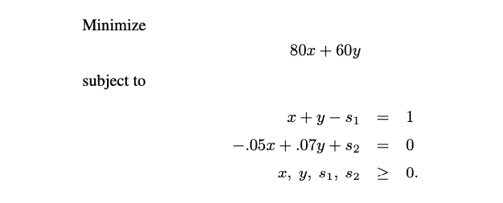
\includegraphics[width=0.8\linewidth]{images/worksheet_6_solution_1.png}
        \end{center}

        \item \textbf{Converting Linear Programming to Standard Form}

        \begin{enumerate}[1)]
            \item The objective function might be a minimization rather than a maximization

            \begin{itemize}
                \item Negate coefficients of the objective function
            \end{itemize}

            \begin{center}
            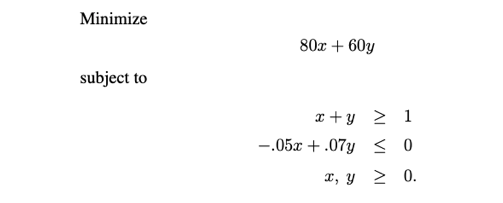
\includegraphics[width=0.9\linewidth]{images/worksheet_6_solution_2.png}
            \end{center}

            \item There might be variables without nonnegativity constraints

            \begin{itemize}
                \item Replace each non-nonnegative variable $x_i$ with $x_i'$ and $x_i''$
                \item Modify linear program
            \end{itemize}

            \begin{center}
            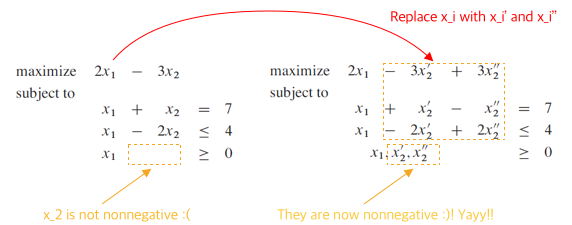
\includegraphics[width=0.9\linewidth]{images/worksheet_6_solution_3.png}
            \end{center}

            \item There might be \textbf{equality constraints}, which have an equal sign rather than a
            less-than-or-equal-to sign

            \begin{itemize}
                \item Replace equality constraint $f(x_1, x_2, ..., x_n) = b$ with
                $f(x_1, x_2, ..., x_n) \leq b$ and $f(x_1, x_2, ..., x_n) \geq b$
            \end{itemize}

            \begin{center}
            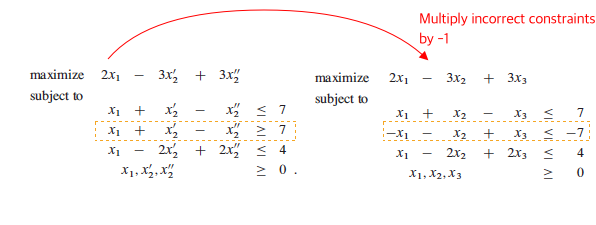
\includegraphics[width=0.9\linewidth]{images/worksheet_6_solution_5.png}
            \end{center}

            \item There might be \textbf{inequality constraints}, but instead of having a less-than-or-equal-to-sign

            \begin{itemize}
                \item Multiply incorrect inequality constraints by -1
            \end{itemize}

            \begin{center}
            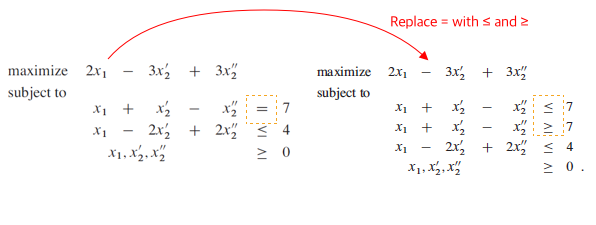
\includegraphics[width=0.9\linewidth]{images/worksheet_6_solution_4.png}
            \end{center}


        \end{enumerate}

    \end{itemize}

    \bigskip

    \underline{\textbf{References:}}

    \bigskip

    \begin{enumerate}[1)]
        \item Wikipedia, Linear Programming, \href{https://en.wikipedia.org/wiki/Linear_programming}{link}
        \item Instituto de Mathematicas, Standard form for Linear Programs, \href{https://www.matem.unam.mx/~omar/math340/std-form.html}{link}
    \end{enumerate}

    \item

    \begin{align*}
        z &= 2x_1 - 6x_3\\
        x_4 &= 7 - x_1 - x_2 + x_3\\
        x_5 &= -8 + 3x_1 - x_2\\
        x_6 &= -x_1 + 2x_2 + 2x_3\\
    \end{align*}

    \bigskip

    The basic variables are variables on the lhs (i.e $B = {4,5,6}$), and the non-basic variables are the
    variables on the rhs of the expressions (i.e. $N = {1,2,3}$).

    \begin{center}
    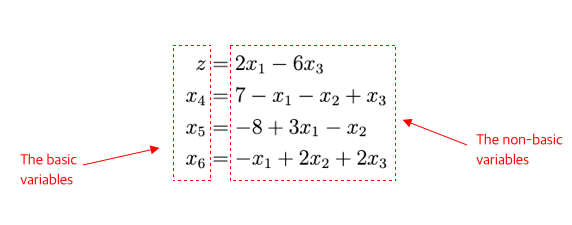
\includegraphics[width=0.7\linewidth]{images/worksheet_6_solution_12.png}
    \end{center}

    \bigskip

    \underline{\textbf{Notes:}}

    \bigskip

    \begin{itemize}

        \item \textbf{Slack Form}

        \begin{itemize}
            \item Is a form of linear programming
            \item Is for efficient solving of liner programming problem using simplex algorithm
        \end{itemize}

        \begin{center}
        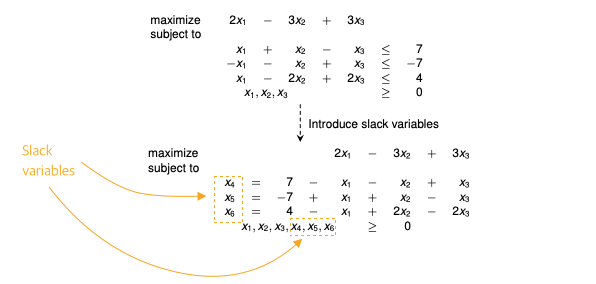
\includegraphics[width=\linewidth]{images/worksheet_6_solution_6.png}
        \end{center}
        \item \textbf{Converting Linear Programs into Slack Form}

        \begin{enumerate}[1)]
            \item Start from the standard form of linear programming
            \item Shift objective functions to right

            \begin{center}
            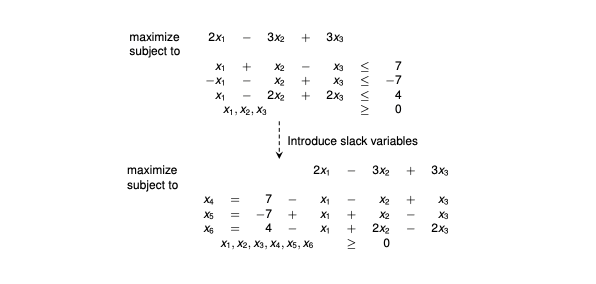
\includegraphics[width=\linewidth]{images/worksheet_6_solution_7.png}
            \end{center}

            \item Introduce slack variable $x_i$ to lhs and move expressions $\sum\limits_{j=1}^n a_{ij}x_j$ to rhs

            \begin{center}
            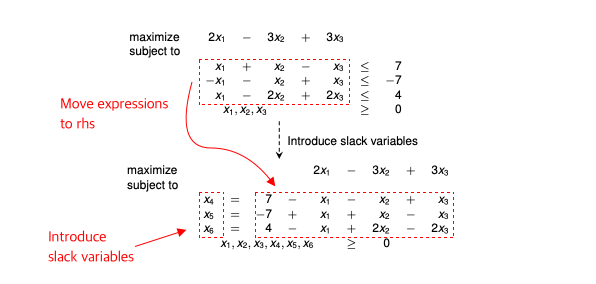
\includegraphics[width=\linewidth]{images/worksheet_6_solution_8.png}
            \end{center}

            \item Change inequalities in linear programming to equality

            \begin{center}
            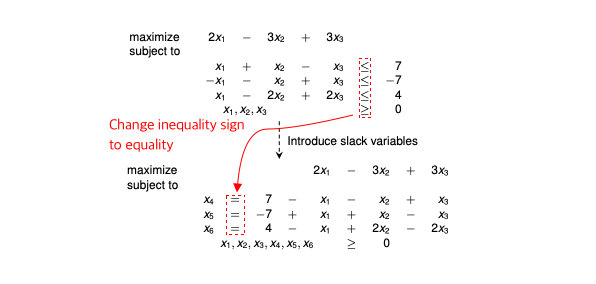
\includegraphics[width=\linewidth]{images/worksheet_6_solution_9.png}
            \end{center}

            \item Use Variable $z$ to denote objective function

            \begin{center}
            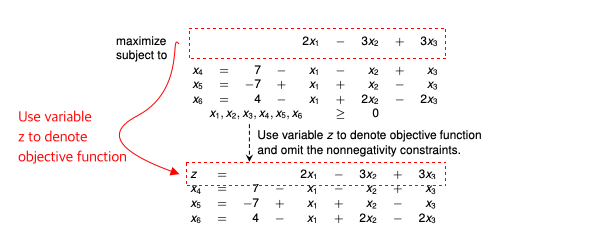
\includegraphics[width=\linewidth]{images/worksheet_6_solution_10.png}
            \end{center}

            \item Omit the nonnegativivty constraints

            \begin{center}
            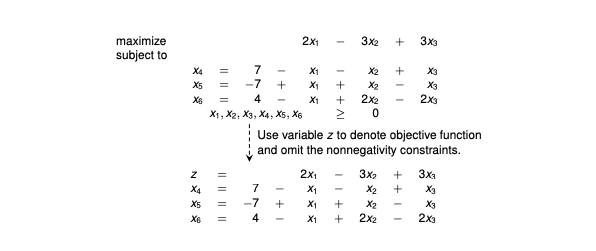
\includegraphics[width=\linewidth]{images/worksheet_6_solution_11.png}
            \end{center}
        \end{enumerate}
    \end{itemize}

    \bigskip

    \underline{\textbf{References:}}

    \bigskip

    \begin{enumerate}[1)]
        \item Cambridge University, Linear Programming, \href{https://www.cl.cam.ac.uk/teaching/1617/AdvAlgo/lp.pdf}{link}
    \end{enumerate}

    \item
    \setcounter{equation}{0}
    \bigskip

    Multiplying the first expression (under subject to) by 2, and summing the inequality constraints,
    we have

    \begin{align}
    0 \leq -6
    \end{align}

    which is impossible.

    \bigskip

    \begin{center}
    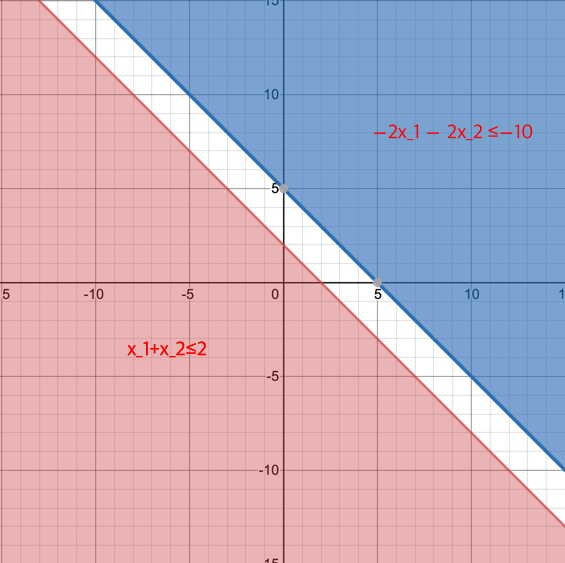
\includegraphics[width=0.5\linewidth]{images/worksheet_6_solution_13.png}
    \end{center}

    \bigskip

    \underline{\textbf{Notes}}

    \bigskip

    \begin{itemize}
        \item I noticed that infeasible solution has non-overlapping region
        \item \textbf{Infeasible}

        \begin{itemize}
            \item A Linear Program is infeasible if there is no solution that satisfies
            all of the constraints
        \end{itemize}
    \end{itemize}

    \item

    \bigskip

    Let $x_1 = 3r$ and $x_2 = r$ where $r \geq 0$. Then the inequality constraints become

    \begin{align*}
        -2 (3r) + (r) = -5r &\leq -1\\
        -(3r) - 2(r) = -5r &\leq -2\\
        3r,r &\geq 0
    \end{align*}

    and are valid.

    \bigskip

    Now, looking at the objective functions, with $x_1 = 3r$ and $x_2 = r$, it
    becomes

    \begin{align*}
        3r - r = 2r
    \end{align*}

    which increases without bound.

    \bigskip

    Thus, there is no maximum, and the linear program is unboudned.

    \bigskip

    \begin{center}
    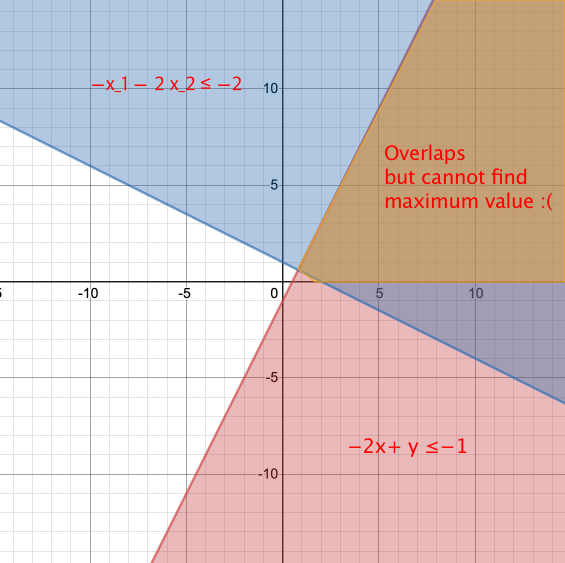
\includegraphics[width=0.5\linewidth]{images/worksheet_6_solution_14.png}
    \end{center}

    % \bigskip

    % \underline{\textbf{Rough Works:}}

    % Let$x_1 = 3r$ and $x_2 = r$ where $r \geq 0$. Then the inequality constraints become

    % \begin{align*}
    %     -2 (3r) + (r) = -5r &\leq -1\\
    %     -(3r) - 2(r) = -5r &\leq -2\\
    %     3r,r &\geq 0
    % \end{align*}

    % and are valid.

    % \bigskip

    % Now, looking at the objective functions, with $x_1 = 3r$ and $x_2 = r$, it
    % becomes

    % \begin{align*}
    %     3r - r = 2r
    % \end{align*}

    % which increases without bound.

    % \bigskip

    % Thus, there is no maximum, and the linear program is unboudned.

    % \bigskip

    % \begin{center}
    % 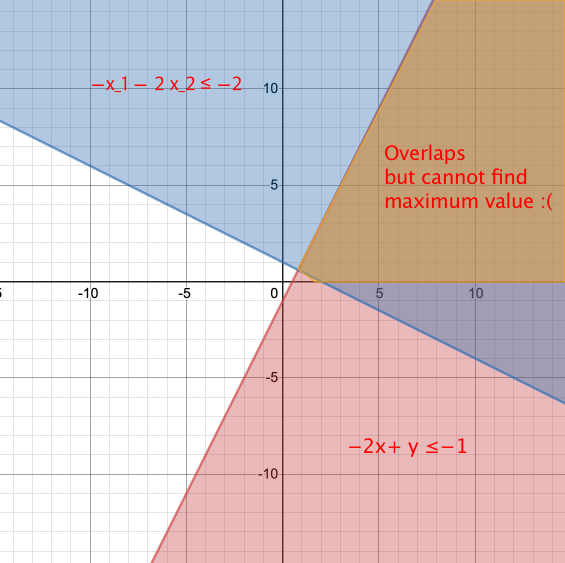
\includegraphics[width=0.5\linewidth]{images/worksheet_6_solution_14.png}
    % \end{center}

    \bigskip

    \underline{\textbf{Notes}}

    \bigskip

    \begin{itemize}
        \item I learned that to show an LP is unbounded, I first have to subtitute
        $x_i$ with a common variable $r$ (e.g. $x_1 = 3r$, $x_2 = r$), check inequality constraints,
        and then look at objective functions and see if I can get max/min.
        \item \textbf{Unbounded}

        \begin{itemize}
            \item A Linear Program is unbounded if it has some feasible solutions but does not
            have a finite optimal objective value
        \end{itemize}
    \end{itemize}

    \bigskip

    \underline{\textbf{References:}}

    \bigskip

    \begin{enumerate}[1)]
        \item CLRS Solutions, 29.1 Standard and slack forms, \href{https://walkccc.github.io/CLRS/Chap29/29.1/}{link}
    \end{enumerate}

    \item

    \bigskip

    At worst case, the upper bound of variables and constraints in conversion to
    standard form is $2n$ and $2m$.

    \begin{proof}

    Suppose a linear program has $n$ variables and $m$ constraints.

    \bigskip

    When converting to standard form, the areas that affect the number of constraints
    and variables are:

    \begin{enumerate}[1.]
        \item Variables without nonnegativity constraints
        \item Existence of equality constraints
    \end{enumerate}

    \bigskip

    So, in worst case, all of the variables are not nonnegative, and all of the
    expressions have equality constraints.

    \bigskip

    Since addressing each of non-nonnegative constraints adds an additional variable,
    we can write there would be total of $2n$ variables at the end.

    \bigskip

    And since addressing each equality constraints result in 1 additional constraint,
    we can conclude there would be total of $2m$ constraints.

    \end{proof}

    \bigskip

    % \underline{\textbf{Rough Works}}

    % \bigskip

    % At worst case, the upper bound of variables and constraints in conversion to
    % standard form is $2n$ and $2m$.

    % \begin{proof}

    % Suppose a linear program has $n$ variables and $m$ constraints.

    % \bigskip

    % When converting to standard form, the areas that affect the number of constraints
    % and variables are:

    % \begin{enumerate}[1.]
    %     \item Variables without nonnegativity constraints
    %     \item Existence of equality constraints
    % \end{enumerate}

    % \bigskip

    % So, in worst case, all of the variables are not nonnegative, and all of the
    % expressions have equality constraints.

    % \bigskip

    % Since addressing each of non-nonnegative constraints adds an additional variable,
    % we can write there would be total of $2n$ variables at the end.

    % \bigskip

    % And since addressing each equality constraints result in 1 additional constraint,
    % we can conclude there would be total of $2m$ constraints.

    % \end{proof}

    \underline{\textbf{References:}}

    \bigskip

    \begin{enumerate}[1)]
        \item CLRS Solutions, 29.1 Standard and slack forms, \href{https://walkccc.github.io/CLRS/Chap29/29.1/}{link}
    \end{enumerate}

    \item

    The following is an example of a linear program for which the feasible region
    is not bounded, but the optimal objective value is finite.

    \bigskip

    Minimum

    \begin{align*}
        x_1 - x_2
    \end{align*}

    Subject to

    \begin{align*}
        -2x_1 + x_2 &\leq -1\\
        -x_1 + 2x_2 &\leq 10\\
        x_1,x_2 &\geq 0
    \end{align*}

    \begin{proof}

    Let $x_1 = 2r$ and $x_2 = r$ where $r \geq 0$. Then, the inequality constraints become


    \begin{align}
        -2(2r) + (r) = -3r &\leq -1\\
        -(2r) + 2(r) = 0 &\leq 10\\
        2r, r &\geq 0
    \end{align}

    which is valid.

    \bigskip

    Now, looking at the objective function, we have $2r - r = r$.

    \bigskip

    Since we are looking for the minimum value and $r \geq 0$, we can write $min(r) = 0$
    (if we are looking for the maximum, then $r$ is ever-increasing and the linear program is unbounded).

    \bigskip

    Thus, the optimal objective value in this example is finite.

    \bigskip

    \begin{center}
    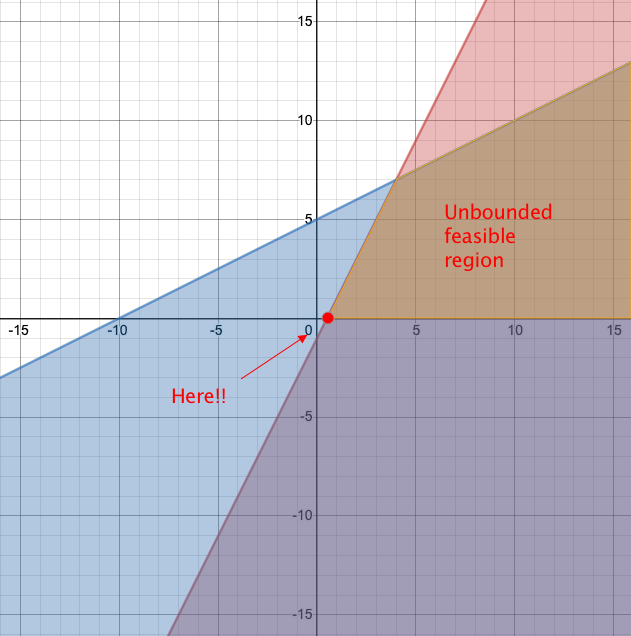
\includegraphics[width=0.5\linewidth]{images/worksheet_6_solution_15.png}
    \end{center}

    \end{proof}

    % \underline{\textbf{Rough Work:}}

    % \bigskip

    % The following is an example of a linear program for which the feasible region
    % is not bounded, but the optimal objective value is finite.

    % \bigskip

    % Minimum

    % \begin{align*}
    %     x_1 - x_2
    % \end{align*}

    % Subject to

    % \begin{align*}
    %     -2x_1 + x_2 &\leq -1\\
    %     -x_1 + 2x_2 &\leq 10\\
    %     x_1,x_2 &\geq 0
    % \end{align*}

    % \begin{proof}

    % Let $x_1 = 2r$ and $x_2 = r$ where $r \geq 0$. Then, the inequality constraints become


    % \begin{align}
    %     -2(2r) + (r) = -3r &\leq -1\\
    %     -(2r) + 2(r) = 0 &\leq 10\\
    %     2r, r &\geq 0
    % \end{align}

    % which is valid.

    % \bigskip

    % Now, looking at the objective function, we have $2r - r = r$.

    % \bigskip

    % Since we are looking for the minimum value and $r \geq 0$, we can write $min(r) = 0$
    % (if we are looking for the maximum, then $r$ is ever-increasing and the linear program is unbounded).

    % \bigskip

    % Thus, the optimal objective value in this example is finite.

    % \bigskip

    % \begin{center}
    % 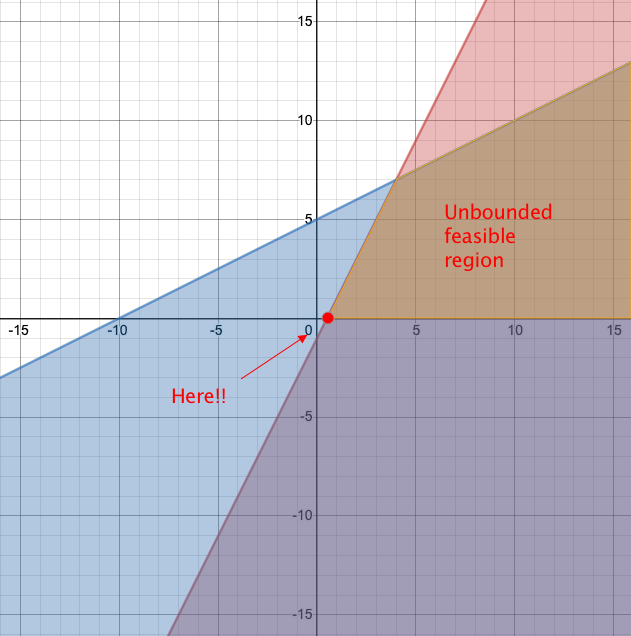
\includegraphics[width=0.5\linewidth]{images/worksheet_6_solution_15.png}
    % \end{center}

    % \end{proof}

    \bigskip

    \underline{\textbf{Notes:}}

    \bigskip

    \begin{itemize}
        \item \textbf{Feasible Region}

        \begin{itemize}
            \item  Is the set of all possible points (sets of values of the choice variables) of an optimization problem that satisfy the problem's constraints. $^{[1]}$
        \end{itemize}
    \end{itemize}

    \underline{\textbf{References:}}

    \bigskip

    \begin{enumerate}[1)]
        \item Wikipedia, Feasible region, \href{https://en.wikipedia.org/wiki/Feasible_region#:~:text=In%20mathematical%20optimization%2C%20a%20feasible,%2C%20equalities%2C%20and%20integer%20constraints.}{link}
    \end{enumerate}


    \item

    \bigskip

    \underline{\textbf{Notes:}}

    \bigskip

    \begin{itemize}
        \item \textbf{Formulating Problems as Linear Program (Shortest Path)}

        \begin{itemize}
            \item Single-source shortest-path problem can be formulated as a linear program.
            \item Goal is computing the weight of a shortest path from $s$ to $t$.
        \end{itemize}
    \end{itemize}


\end{enumerate}

\end{document}